%%%%%%%%%%%%%%%%%%%%%%%%%%%%%%%%%%%%%%%%%%%%%%%%%%%%%%%%%%%%%%%%%%%%%%%%%%%%%%%%
\documentclass[
preprint,          % 12pt, single-column
superscriptaddress,% authors with affiliations via superscripts
amsmath,           % add AMS-Latex features
amssymb,           % add extra AMS symbols, including amsfonts
aps,               % aps or aip
prl,               % prl, pra, prb, prc, prd, pre, prstab
notitlepage,       % control appearance of title page
longbibliography,  % show  article titles in the bibliography
floatfix,          % process floats as early as possible
nofootinbib,
onecolumn,
]{revtex4-1}

\usepackage{bm}         % \bm{<text>} Bold math symbols
\usepackage{amsmath}
\usepackage{graphicx}   % include figures
\usepackage[
colorlinks=true,        % color link
citecolor=blue,         % cite color
linkcolor=blue,         % link color
urlcolor=blue           % url color
]{hyperref}             % create hyperlinks
\usepackage{color}    
\newcommand{\nc}{\newcommand*} 
\nc{\fpbh}{f_{\mathrm{pbh}}}    % f_pbh
\nc{\Mmin}{{M_{\mathrm{min}}}}
\nc{\Mf}{{M_\mathrm{f}}}
\nc{\al}{\alpha}
\newcommand{\red}[1]{\textcolor{red}{#1}}

\newcommand{\cR}{\mathcal{R}}

\begin{document}

\noindent Response to Report of the Referee -- DY12741/Liu\\

We would like to thank the referee for the valuable comments and suggestions. We have considered all of them and revised the manuscript accordingly.
Our responses to the comments are given below.

\begin{enumerate}
	
\item \red{\it My first general question is whether it is really necessary to perform a detailed analysis to know that the second-generation merger can be neglected? To me the neglected contribution is definite from a back-of-the-envelope calculation, given the current knowledge that the fraction of PBH in dark matter $f_{pbh}$ is O($10^{-3}$). I read with interest the authors' previous event rate modeling paper ref. 21 that the current manuscript heavily relies on. Using the binary formation criteria Eq. 1 of ref. 21, that $x^3$ $n_{pbh}$ should $<$ $f_{pbh}$ (I reckon $x^3$ the occupation volume of a PBH and $1/n_{pbh}$ is the average volume occupied by a PBH), I estimate a fraction of $O(f_{pbh})$ formed binaries. The reasoning is that I made the (crude) assumption that $x^3$ is uniformly distributed within $[0, 1/n_{pbh}]$, thus only a fraction $f_{pbh}$ satisfies the condition. A more practical distribution for x was also given by ref. 21 and should give a more precise estimation. This work concluded the second-generation merger contributes $10^{-2}$ to the first-generation, not $10^{-3}$, but the crude estimation for x and assuming a single-mass may cause the difference. Anyway, my point is that the authors may be able to estimate the order of magnitude of second-generation mergers, given a nice analytical model of merger rate and knowledge about $f_{pbh}$. Does this make sense? Putting it in another way, in the section of the assessment, I was asked to evaluate whether this paper yields significant new physics results to warrant publication, so I'm trying to understand how innovative this manuscript's result is. If the numerical analysis performed by this manuscript can offer more insights about the second-generation merger (not just confirming what was expected with more precise digits), I would consider the results more innovative.}

First of all, we respectfully disagree with some points of the referee as we believe there may be some misunderstandings. Eq.~1 of ref.~21 is the condition for black holes to form binaries, but not the condition to form second-generation binaries. The fraction of the second-generation merger rate over the first-generation merger rate should be given by Eq.~(7) over Eq.~(5). We note that the fraction depends not only on $f_{pbh}$ and the mass function, but also on the cosmic time (or redshift); and the fraction will increase as cosmic time increases.

Secondly, compared to GWTC-1, GWTC-3 has greatly enlarged the number of BBH events. Most importantly, GWTC-3 contains much more heavy black holes and shifts the mass distribution of black holes to a larger value. This motivates us to investigate whether these heavy black holes are (partly) formed from second-generation mergers or not, since the second-merger process will shift the mass distribution to a larger value. Although we agree that the merger rate from second-merger process cannot make significant contribution even from a crude estimation, an accurate estimation of the impact of the second-merger process on the mass distribution should come from careful data analyses as done in this work. In fact, as can be seen Fig.~(8), the second-merger process can significantly shift the mass distribution to heavy mass as $\cR_2/\cR_1$ can be $\geq 50\%$.

In summary, we believe our work has considerable significance and novelty. Moreover, in the revised version of the manuscript, we have added some sentences to explain our novelty in the Introduction.

\item \red{\it My second question concerns the fact that this manuscript didn't consider the PBH cluster at the late time of the universe, rather it still reckons the second-generation merger from spatially uniformly distributed PBHs. At late times the dark matter forms halo structures, thus causing the PBH to cluster, and thus maybe boosting the merger rate. This was considered e.g. by 2012.02786 (see their $S_2$ term). Can this effect be safely ignored by the current work?}

We would like to thank the referee for pointing out this effect as well as the reference 2012.02786. Yes, this effect can be safely ignored. According to Ref.~\cite{Hutsi:2020sol}, the suppression factor $S_2(z,f_{\mathrm{pbh}})$ can be approximated as 
\begin{equation}
    S_2(z,f_{\mathrm{pbh}}) \approx \mathrm{min}[1,\Tilde{S_2}(z,f_{\mathrm{pbh}})], 
\end{equation}
where 
\begin{equation}
\Tilde{S_2}(z,f_{\mathrm{pbh}})=9.6 \times 10^{-3} {\left(\left(t[z]/t_0\right)^{0.44}f_{\mathrm{pbh}}\right)}^{-0.65} e^{0.03 \ln ^2 \left(\left(t[z]/t_0\right)^{0.44}f_{\mathrm{pbh}}\right)},
\end{equation}
which decrease as $f_{\mathrm{pbh}}$ increase and increase as $z$ increase. For all of the four PBH mass functions, we always have $f_{\mathrm{pbh}} \lesssim 3\times10^{-3}$. Therefore, we always have $\Tilde{S_2}(z,f_{\mathrm{pbh}})\geq \Tilde{S_2}(0,3\times 10^{-3}) \approx 1.15$ and $S_2(z,f_{\mathrm{pbh}})\approx 1$. As a result, this effect can be safely ignored.  In the revised version, we have cited this reference and added the following discussion in the Conclusion section:

\textit{``PBHs cluster at the late time of the Universe may play an important role in the merger rate. For all of the four PBH mass functions, we always have $f_{\mathrm{pbh}} \lesssim 3\times10^{-3}$. Therefore, according to Ref.~\cite{Hutsi:2020sol}, this effect can be safely ignored."}


%Yes, this effect can be safely ignored. For all of the four PBH mass functions, we always have $f_{\mathrm{pbh}} \in [10^{-3},3\times10^{-3}]$, and therefore $S_2[z]\approx 1$ as shown in the following figure. I would like to thank the referee for pointing out this effect as well as the reference 2012.02786. In the revised version, we have cited this reference and added the following discussion in the Conclusion section:


\item \red{\it The title remains ``Constrain ..." in the manuscript, but in the PRD submission system it has been changed to ``Constraining ...". Keep the latter.}

We thank the referee for pointing out this inconsistency. We have changed the title to ``Constraining ..." in the revised version.


\item \red{\it Section 1: The first paragraph, the second last sentence ``even accounting for the uncertainties in modelling...", I think the authors meant ``statistical uncertainties" (i.e., the uncertainty of parameter estimation). Other models exist for GW190521, such as eccentric orbits, hyperbolic encounters models, or even proca star head-on collisions. In those models, especially the proca star, the mass in the gap may not be the case.}

Yes, we meant ``statistical uncertainties", and we have rephrased the sentence as ``even accounting for the statistical uncertainties, it ...".

\item \red{\it Section 1: paragraph 3, in the middle, ``we use GWTC-3, which expands GWTC-1 with almost six times", add that the GWTC-3 is purified by using a subset. I was confused at the first pass why it was not nine times more.}

We have rephrased it as ``we use a purified subset of GWTC-3, which expands GWTC-1 with almost six times".

\item \red{\it Although the authors recommended the readers to ref 21 for details, this manuscript should add more descriptions to at least explain all terms. For example, I couldn't find the meaning of $m_i$, $m_j$ and $m_l$, $m_e$, etc.}

In the revised version, we have added more descriptions to explain all terms, including $m_i$, $m_j$, $m_l$, and $m_e$, etc., as suggested by the referee.

\item \red{\it Under equation 4, ``the PBHs are randomly distributed", add ``following a spatial Poisson distribution" otherwise it's not clear what is the random distribution. Also, ``These two PBH would ... and form a PBH binary", add the condition to form a binary, i.e., decouple from the cosmic expansion.}

As suggested by the referee, we have rephrased these two sentences as 1) ``the PBHs are randomly distributed following a spatial Poisson distribution ..."; 2) ``These two PBH would ... and form a PBH binary after decoupling from the cosmic expansion".

\item \red{\it Under equation 8 the authors only considered the merger history up to the second, is it because the authors have estimated the third merger and know it can be safely neglected? To echo my first question, can the authors also estimate the contribution from the second merger along the same line?}

Yes, we have estimated the effect of the third-merger process. Based on best-fit parameter values inferred from both the first- and second-merger, we found the contribution from the third merger can be negligible as can be seen from the following figure. In fact, we have $\cR_3/\cR_2 \leq 0.005$ for the critical collapse mass function.

\begin{figure}[hp!]
	\centering
	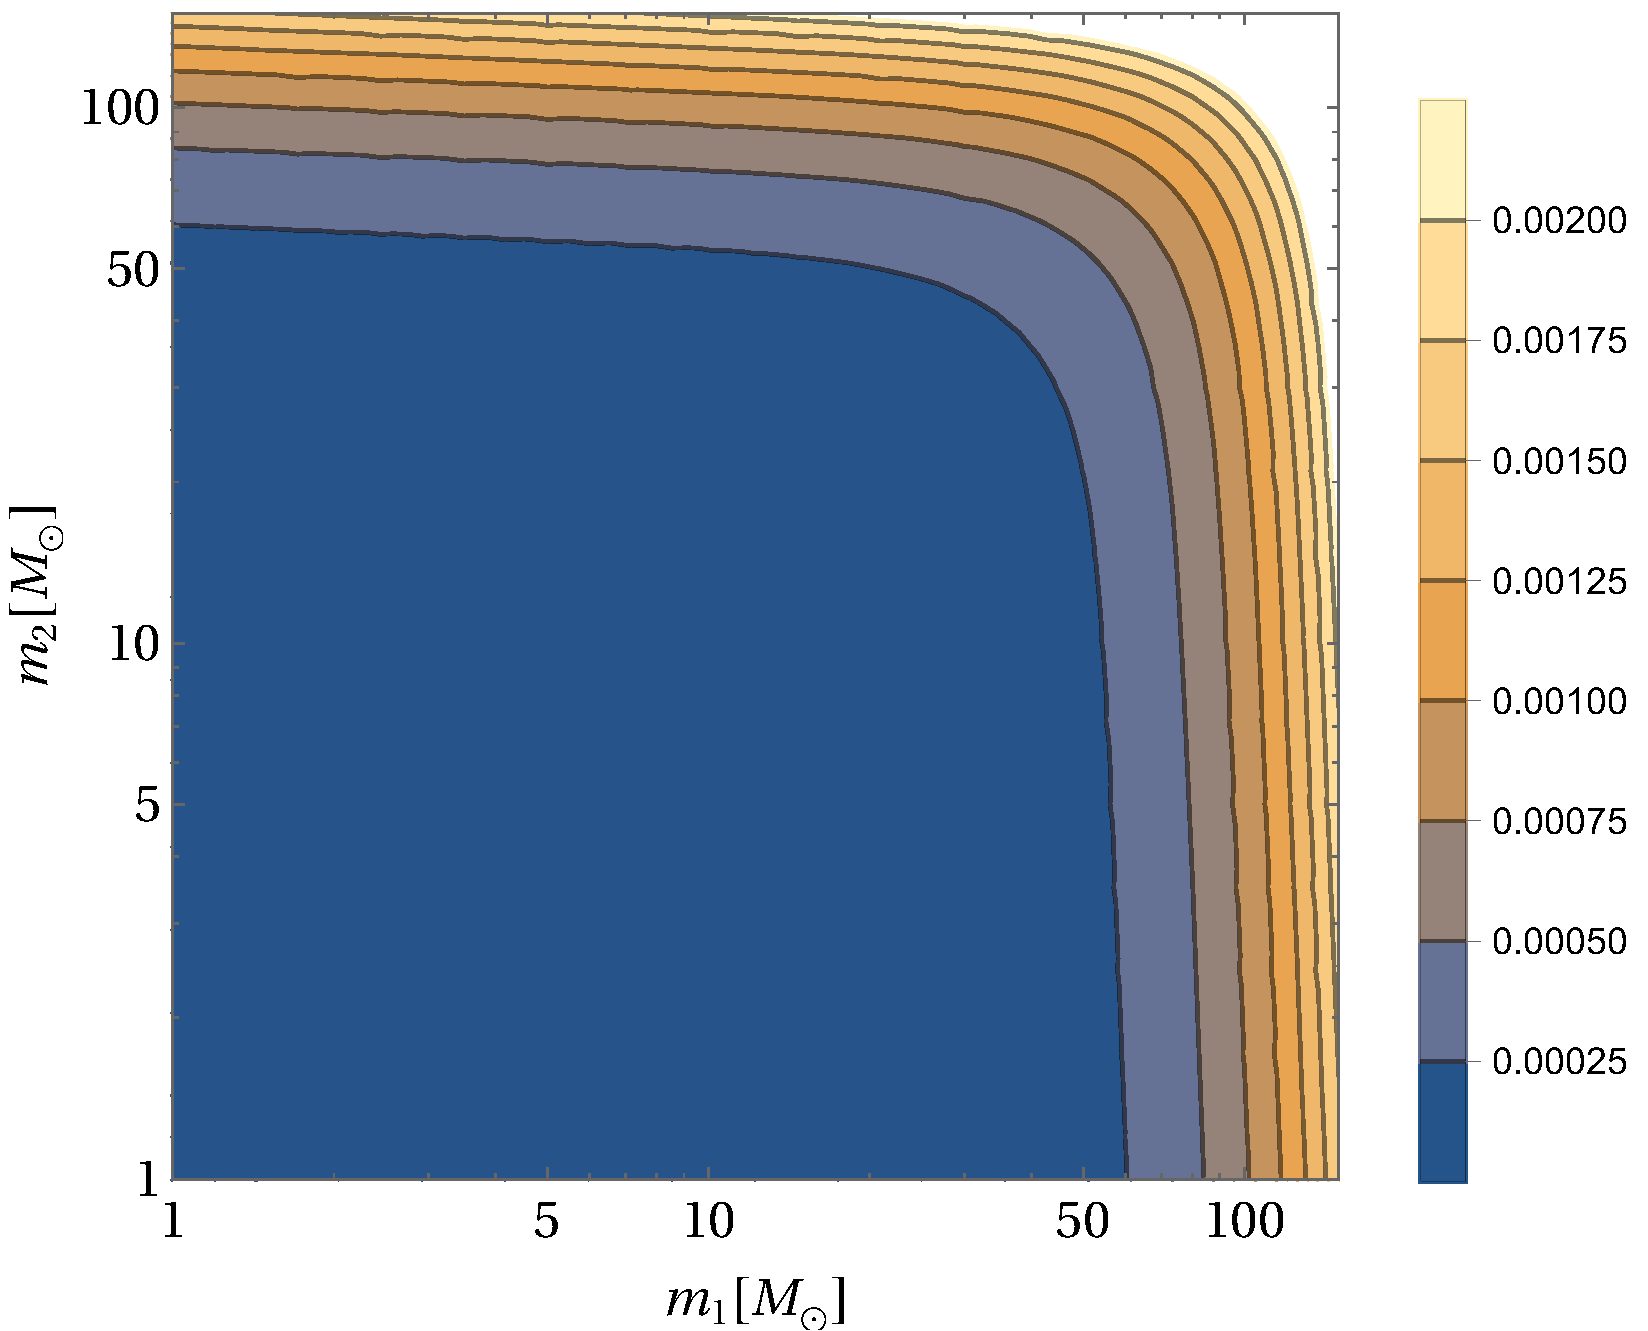
\includegraphics[width=0.6\textwidth]{ratio-CC-32.pdf}
	\caption{\label{ratio-power}The ratio of merger rate density from the third merger to that from the second merger, $\cR_3(t_0, m_1, m_2)/\cR_2(t_0, m_1, m_2)$, as a function of component masses for the critical collapse mass function. We have fixed the hyper-parameters $\{\Mf, \al, \fpbh\}$ to their best-fit values.}
\end{figure}

However, the second-merger process can significantly shift the mass distribution to heavy mass as $\cR_2/\cR_1$ can be $\geq 50\%$ for the critical collapse mass function as can be seen from Fig.~(8) in the manuscript.

\item \red{\it Conclusion: The second paragraph said ``Therefore the merger history of PBH binaries has a sub-dominant effect...", I suggest making it clear that by ``merger history" the authors really meant the higher-order hierarchical merger after the first one. My reasoning is that the term "merger history" may be confused by the PBH merger rate as a function of different cosmic time.}

As suggested by the referee, we have rephrased the sentence as ``Therefore the higher-order hierarchical merger after the first one has a sub-dominant effect...".

\end{enumerate}

We have highlighted the changes in the bold font in the manuscript. We hope these changes will address the referee's concerns. Please reconsider our paper for publication in PRD. \\

\noindent Sincerely,\\
Lang~Liu, Zhi-Qiang~You, You~Wu, Zu-Cheng~Chen

%%%%%%%%%%%%%%%%%%%%%%%%%%%%%%%%%%%%%%%%%%%%%%%%%%%%%%%%%%%%%%%%%%%%%%%%%%%%%%%%
%%%%%%%%%%%%%%%%%%%%%%%%%%%%%%% %%% references %%%%%%%%%%%%%%%%%%%%%%%%%%%%%%%%%%
\bibliography{ref}
%%%%%%%%%%%%%%%%%%%%%%%%%%%%%%%%%%%%%%%%
\end{document}

%%%%%%%%%%%%%%%%%%%%%%%%%%%%%%%%%%%%%%%%

